\chapter{Tinjauan Pustaka}

\section{Studi Terkait}
\blindtext

\section{Dasar Teori}
Penelitian ini menggunakan beberapa teori dasar pendukung agar dapat memperjelas proses penelitian dan memberikan pemahaman lebih lanjut. Teori-teori dasar yang berhubungan dan digunakan dalam penelitian ini adalah sebagai berikut.
\subsection{MapReduce}
MapReduce adalah model pemrograman dan implementasi teknik pemrosesan data berukuran besar yang pertama kali dipopulerkan oleh Google pada tahun 2004\cite{kaliaAnalysisHadoopMapReduce2021}. MapReduce menawarkan pemrosesan data yang dapat diandalkan serta \textit{fault-tolerant manner} (tahan terhadap kesalahan).  MapReduce berjalan secara paralel dan berada pada lingkungan komputasi terdistribusi \cite{cTaskFailureResilience2020}. Model ini mengadopsi arsitektur tersentraliasi, yaitu satu \textit{node} berperan sebagai \textit{master} dan \textit{node} yang lain berperan sebagai \textit{workers} atau \textit{slave} \cite{herodotouHadoopPerformanceModels2011, bakratsasHadoopMapReducePerformance2018}. \textit{Master node} bertanggung jawab untuk melakukan penjadwalan kerja, dan \textit{slave node} berperan untuk menjalankan eksekusi kerja. 

\begin{figure}[h!]
    \centering
    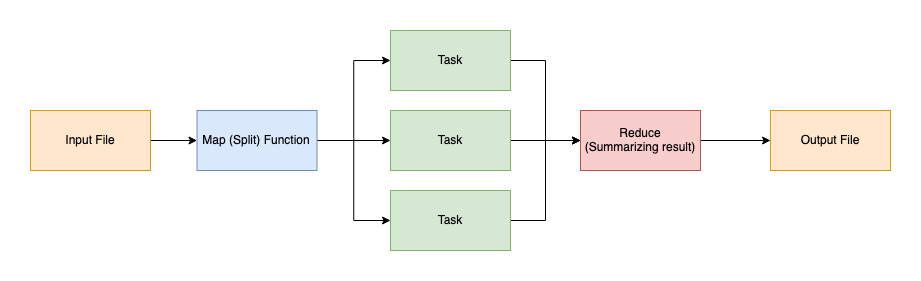
\includegraphics[width=1\textwidth]{figures/ch02/mapreduce-scheme.png}
    \caption{Cara Kerja MapReduce}
    \label{fig:mapreduce-flow}
\end{figure}

MapReduce terdiri dari fungsi \textit{Map} dan fungsi \textit{Reduce} \cite{gandomiHybSMRPHybridScheduling2019}. Kedua fungsi ini tersebar di seluruh \textit{slave node} yang terhubung dalam klaster dan berjalan secara paralel. Fungsi \textit{Map} berperan untuk membagi masalah besar menjadi masalah yang lebih kecil dan mendistribusikannya ke \textit{slave node}. Hasil pemrosesan dari \textit{slave node} akan dikumpulkan oleh \textit{master node} melalui fungsi \textit{Reduce}. Sesuai dengan Gambar \ref{fig:mapreduce-flow}, hasil dari proses \textit{Reduce} yang akan dikirimkan sebagai hasil akhir proses MapReduce.  

Implementasi MapReduce pada \textit{Word Count}\cite{KOMPARASIKECEPATANHADOOP} dapat dilihat pada Gambar \ref{fig:mapreduce-wordcount}. Pada proses MapReduce, data masukan akan melalui beberapa tahapan pemrosesan. Pertama, data akan dipecah menjadi bagian-bagian yang lebih kecil pada proses pemecahan data masukan (\textit{splitting}). Dalam kasus Hadoop MapReduce, data idealnya akan dipecah menjadi beberapa blok berukuran maksimal 128MB.

\begin{figure}[h!]
    \centering
    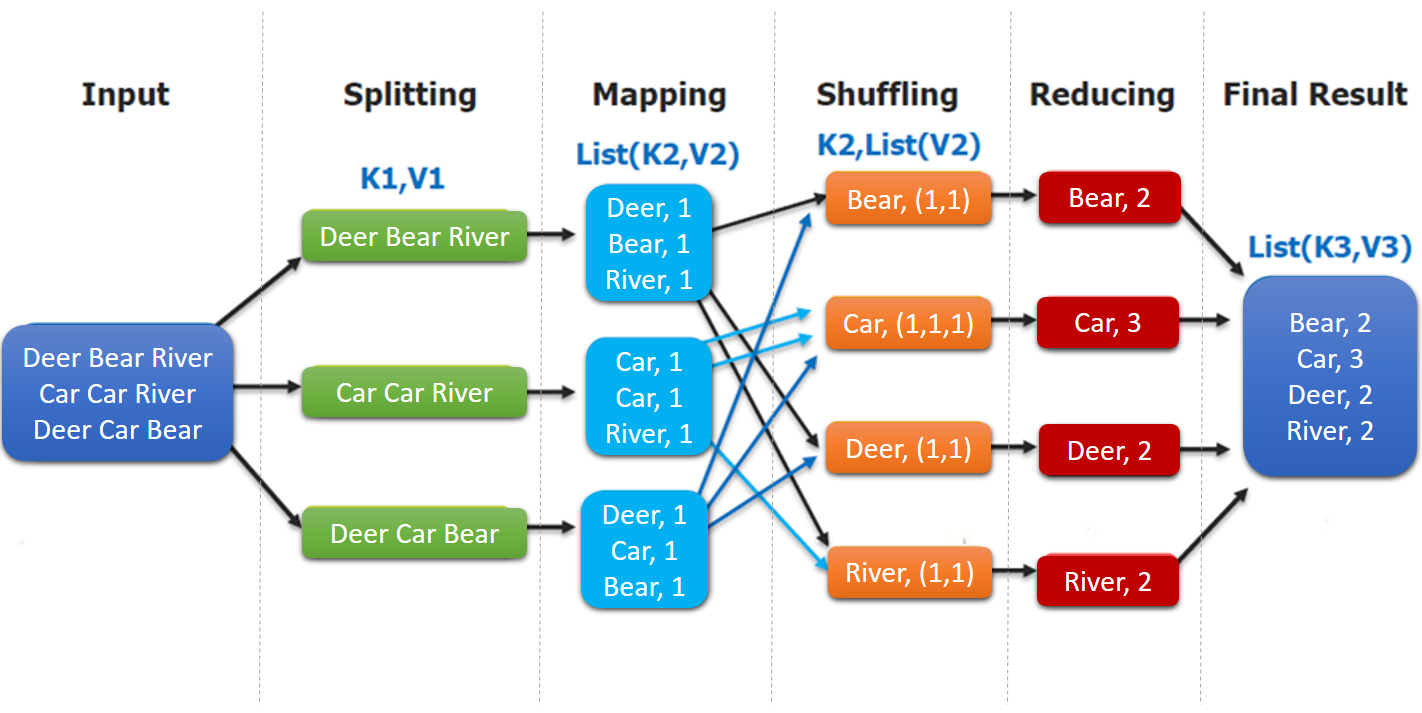
\includegraphics[width=0.9\textwidth]{figures/ch02/map-reduce-word-count-oreilly.png}
    \caption{Implementasi MapReduce pada Word Count. Sumber:  \cite{MapReduceDistributedComputing}}
    \label{fig:mapreduce-wordcount}
\end{figure}

Kemudian, blok data tersebut akan diproses lebih lanjut pada tahap pemetaan (\textit{mapping}). Pemetaan merupakan salah satu tahapan terpenting dalam MapReduce. Pada tahap ini, blok data yang sudah dipecah akan diproses untuk menghasilkan pasangan kunci-nilai (\textit{key-value pairs}) sementara, seperti pada contoh kasus \textit{wordcount} yang menghasilkan pasangan kunci-nilai \textit{Dear:1, Bear:1, dan River:1}. Pemetaan dapat melibatkan satu atau beberapa mesin pekerja (\textit{worker}) yang memproses blok data secara paralel.

Selanjutnya adalah tahap pengocokan (\textit{shuffling}) di mana pasangan kunci-nilai hasil pemetaan yang tersebar di beberapa mesin akan dikumpulkan berdasarkan kesamaan kuncinya agar bisa diproses lebih lanjut. Misalnya semua pasangan dengan kunci \textit{Bear} dikumpulkan dalam satu mesin.

Pada tahap terakhir yaitu pengurangan (\textit{reducing}), dilakukan agregasi terhadap pasangan kunci-nilai dengan kunci yang sama untuk menghasilkan keluaran akhir. Seperti pada contoh kasus \textit{wordcount}, pasangan \textit{Bear:1} dan \textit{Bear:1} akan dijumlahkan menjadi \textit{Bear:2} oleh proses pengurangan.

\subsection{Apache Hadoop}
Apache Hadoop adalah perangkat lunak sumber terbuka yang ditulis dengan bahasa pemrograman Java untuk pemrosesan dan penyimpanan data menggunakan komputasi terdistribusi (\cite{ApacheHadoop}). Hadoop dapat diinstalasi pada satu \textit{node} komputer, atau ratusan \textit{node} komputer yang digabungkan dalam sebuah klaster (\cite{maneasEvolutionHadoopDistributed2018}). Berkaitan dengan pemrosesan data, Hadoop mengimplementasikan model MapReduce untuk pemrosesan data secara paralel dan cepat. Selain itu, Hadoop menyediakan sistem penyimpanan data terdistribusi yang dikenal sebagai Hadoop Distributed File System (HDFS) untuk akses data, pemrosesan, dan komputasi \cite{dabasAnalysisCommentsYoutube2019}. Arsitektur Hadoop secara umum dapat dilihat pada Gambar \ref{fig:hadoop-str}.

\begin{figure}[h!]
    \centering
    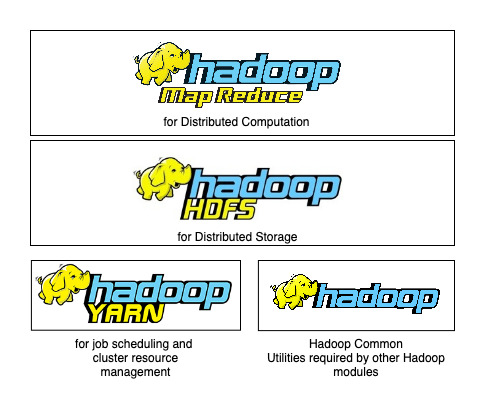
\includegraphics[width=0.9\textwidth]{figures/ch02/hadoop-str}
    \caption{Arsitektur Hadoop}
    \label{fig:hadoop-str}
\end{figure}



\subsubsection{Cara Kerja Apache Hadoop}
\blindtext
\subsubsection{Hadoop Distributed File System (HDFS)}
\blindtext
\subsubsection{Hadoop Map Reduce}
\blindtext
\subsection{Apache Spark}
\blindtext
\subsection{HiBench Suite}
\blindtext
\subsubsection{Jenis-jenis Beban Kerja pada HiBench}